\documentclass[12pt]{article}

% This first part of the file is called the PREAMBLE. It includes
% customizations and command definitions. The preamble is everything
% between \documentclass and \begin{document}.

\usepackage[margin=1in]{geometry}  % set the margins to 1in on all sides
\usepackage{graphicx}              % to include figures
\usepackage{amsmath}               % great math stuff
\usepackage{amsfonts}              % for blackboard bold, etc
\usepackage{amsthm}                % better theorem environments
\usepackage{amssymb} 
\usepackage{mathptmx}
\usepackage{graphicx}
\usepackage{enumerate}
\usepackage{listings}
\usepackage{xcolor}
\usepackage{array}

% various theorems, numbered by section

\newtheorem{thm}{Theorem}[section]
\newtheorem{lem}[thm]{Lemma}
\newtheorem{prop}[thm]{Proposition}
\newtheorem{cor}[thm]{Corollary}
\newtheorem{conj}[thm]{Conjecture}
\newtheorem{mydef}[thm]{Definition}


\lstset{
	basicstyle          =   \sffamily,          
	keywordstyle        =   \bfseries,          
	commentstyle        =   \rmfamily\itshape,  
	stringstyle         =   \ttfamily,  
	flexiblecolumns,                
	numbers             =   left,   
	showspaces          =   false,  
	numberstyle         =   \fontsize{5}{skip},    
	showstringspaces    =   false,
	captionpos          =   t,      
	frame               =   lrtb,   
}

\lstdefinestyle{cpp}{
	language        =   cpp, 
	basicstyle      =   \fontsize{5}{skip},
	numberstyle     =   \fontsize{5}{skip},
	keywordstyle    =   \color{blue},
	keywordstyle    =   [2] \color{teal},
	stringstyle     =   \color{magenta},
	commentstyle    =   \color{red}\ttfamily,
	breaklines      =   true,   
	columns         =   fixed,  
	basewidth       =   0.5em,
}
\begin{document}


\title{ CSE 102 Spring 2021\\
	Advanced Homework Assignment 7}

\author{Jaden Liu \\ 
University of California at Santa Cruz\\
Santa Cruz, CA 95064 USA }

\maketitle


\section{AdvHW7} 
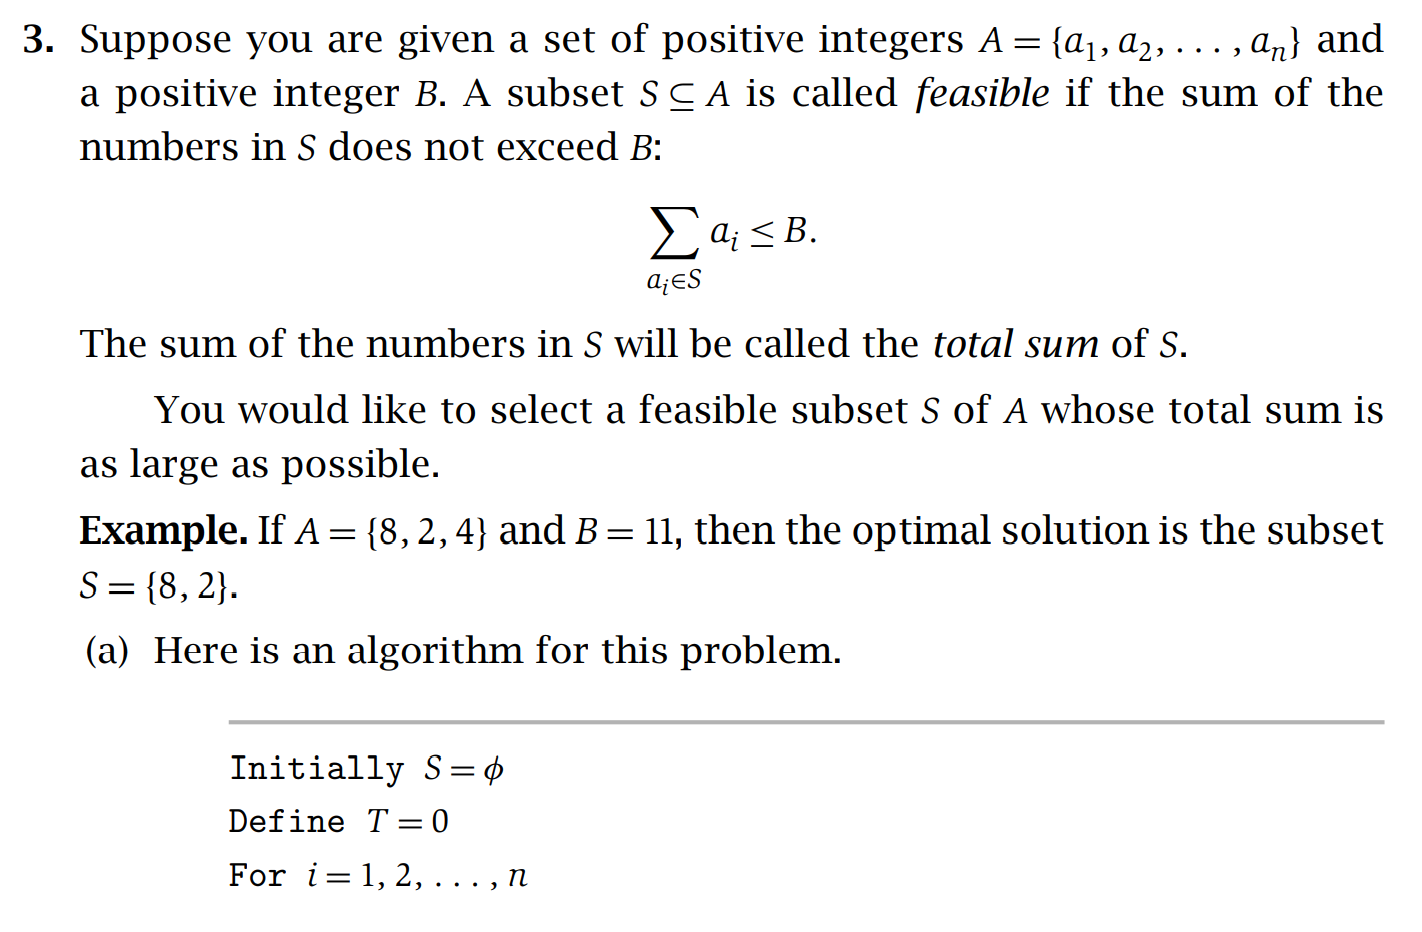
\includegraphics[scale=0.25]{adv_10.png}\\
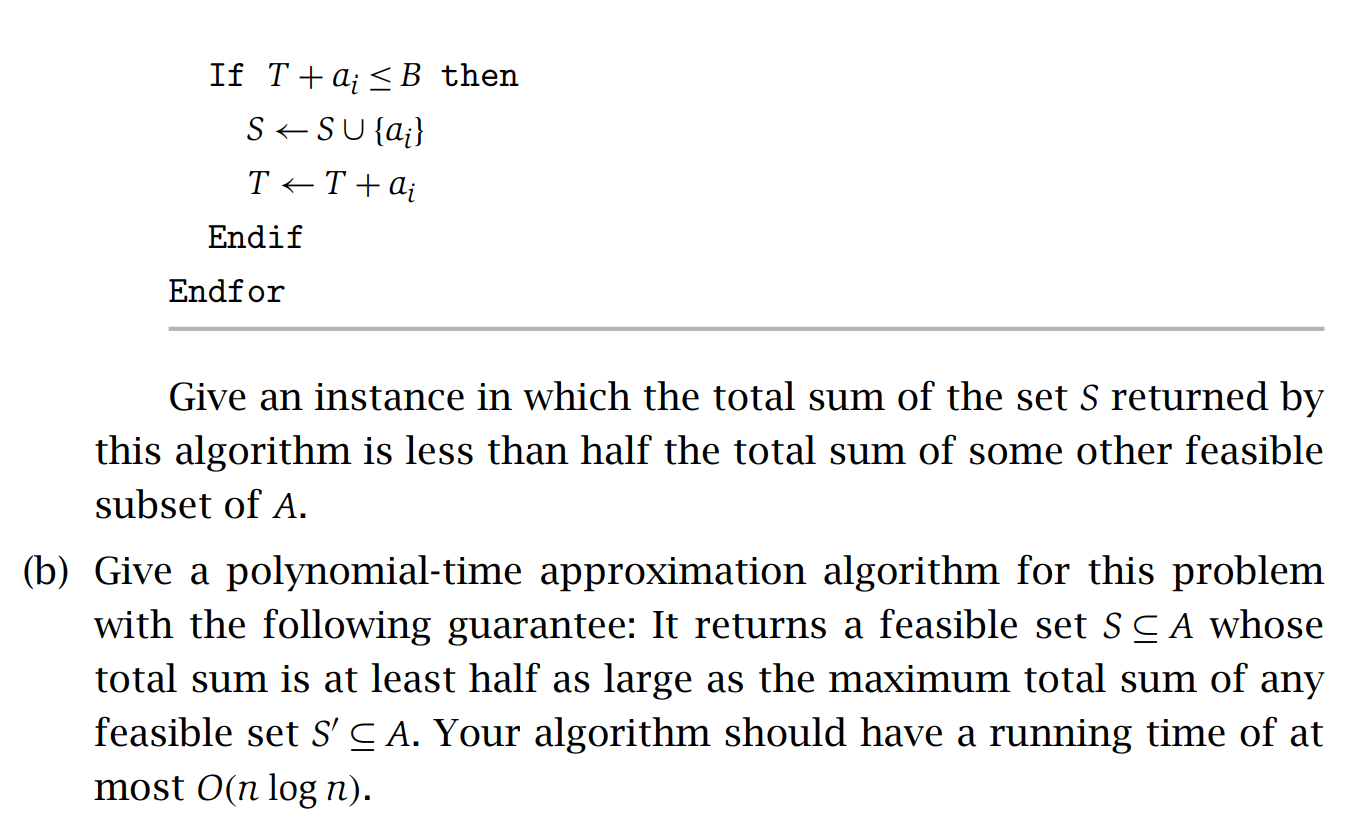
\includegraphics[scale=0.25]{adv_10_2.png}\\
\begin{proof}[Solution for a]
	Assume we have A = \{2,4,10\} and B = 15, which is similar to the above problem. Then we first pick 2, then 4, but we cannot pick 8 since it's overloaded. Then we have our solution S = \{2,4\}, which is smaller than the optimal solution $S_{opt}$ = \{10,4\}, and $S_{sum}=6<\frac{1}{2}S_{optsum}=\frac{1}{2}*14$.
\end{proof}
\begin{proof}[Algorithm]
	1. Order the inputs set A by descending value;\\
	2. Put the next-largest input into the subset, as long as it won't over limit.\\
	The time complexity for the first step(using quick sort or merge sort) is O(nlogn). The second step is O(n) since we need to add every input and compare them. Thus the total running time is at most O(nlogn).\\
\end{proof}
\begin{proof}[Proof for 2 approximation]
	When this algorithm terminate, there are two situation:
	
	1. We have put every element in A to the S, then obviously it has been the optimal solution.
	
	2. We have an input element that cannot fit in the set S, hence we terminated.\\
	For the second situation, we name the first such input as $a_i$. Then we have $a_1+a_2+\cdots+a_{i-1}+a_{i}>S_{optsum}$. Since A is in descending order, then $a_1+a_2+\cdots+a_{i-1}>a_i$, $2(a_1+a_2+\cdots+a_{i-1})>a_1+a_2+\cdots+a_{i-1}+a_{i}>S_{optsum}$. Thus, we proved that $a_1+a_2+\cdots+a_{i-1}>\frac{1}{2}S_{optsum}$, which means our greedy solution will be at least half as large as the optimal maximum total sum.
\end{proof}



\end{document}
